% Part: sets-functions-relations
% Chapter: infinite
% Section: hilberts-hotel
%
\documentclass[../../../include/open-logic-section]{subfiles}

\begin{document}

\olfileid{sfr}{infinite}{hilbert}
\olsection{Hilbert's Hotel}

The set of the natural numbers is obviously infinite. So, if we do not
want to \emph{help ourselves} to the natural numbers, our first step
must be characterize an infinite set in terms that do not require
mentioning the natural numbers themselves. Here is a nice approach,
presented by Hilbert in a lecture from 1924. He asks us to imagine
\begin{quote}
[\ldots] a hotel with a finite number of rooms. All of these rooms
should be occupied by exactly one guest. If the guests now swap their
rooms somehow, [but] so that each room still contains no more than one
person, then no rooms will become free, and the hotel-owner cannot in
this way create a new place for a newly arriving guest [\ldots
\textparagraph \ldots]

Now we stipulate that the hotel shall have infinitely many numbered
rooms $1$, $2$, $3$, $4$, $5$, \dots, each of which is occupied by
exactly one guest. As soon as a new guest comes along, the owner only
needs to move each of the old guests into the room associated with the
number one higher, and room~$1$ will be free for the newly-arriving
guest. 
	\begin{center}
		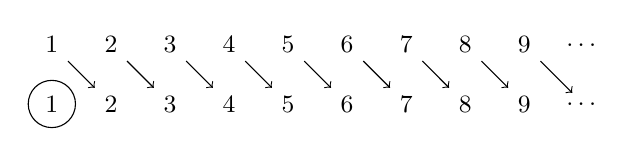
\begin{tikzpicture}[scale = .75]
		\foreach \x in {1, 2, 3, 4, 5, 6, 7, 8, 9}
		{
			\node (\x a) at (\x, 1) {\small{\x}};
			\node (\x b) at (\x, 2) {\small{\x}};
		}
		\node (dotsa) at (10, 1) {\small{\ldots}};
		\node (dotsb) at (10, 2) {\small{\ldots}};
		\draw[->] (1b)--(2a);
		\draw[->] (2b)--(3a);
		\draw[->] (3b)--(4a);
		\draw[->] (4b)--(5a);
		\draw[->] (5b)--(6a);
		\draw[->] (6b)--(7a);
		\draw[->] (7b)--(8a);
		\draw[->] (8b)--(9a);
		\draw[->] (9b)--(dotsa);
		\draw (1,1) circle (.4);
		\end{tikzpicture}
	\end{center}
	(published in \citealt[730]{EwaldSieg2013}; our translation)
\end{quote}
The crucial point is that Hilbert's Hotel has infinitely many rooms;
and we can take his explanation to define what it means to say this.
Indeed, this was Dedekind's approach (presented here, of course, with
massive anachronism; Dedekind's definition is from
\citeyear{Dedekind1888}):

\begin{defn}\ollabel{defn:DedekindInfinite}
A set $A$ is \emph{Dedekind infinite} iff there is !!a{injection}
from~$A$ to a proper subset of~$A$. That is, there is some $o \in A$
and !!a{injection} $f \colon A \to A$ such that $o \notin \ran{f}$.
\end{defn}

\end{document}